\documentclass[a4paper,11pt]{amsart}

\usepackage{a4wide}
\usepackage{amsmath}
\usepackage{amssymb}
\usepackage{amsthm}
\usepackage[czech]{babel}
\usepackage{bookmark}
\usepackage{enumerate}
\usepackage[T1]{fontenc}
\usepackage{forest}
\usepackage{hyperref}
\usepackage[utf8]{inputenc}
\usepackage{lmodern}
\usepackage{multicol}
\usepackage{tikz}

\theoremstyle{definition}
    \newtheorem{problem}{Příklad}

% \theoremstyle{remark}
%     \newtheorem*{steps}{Postup řešení}

\theoremstyle{plain}
    \newtheorem*{solution}{Řešení}
    

\DeclareRobustCommand\proves{\mathrel{|}\joinrel\mkern-.5mu\mathrel{-}}
\DeclareMathOperator{\Conseq}{Csq}
\DeclareMathOperator{\M}{M}

% hide solutions
\newif\ifhidesolutions
    \hidesolutionstrue
    % \hidesolutionsfalse

\ifhidesolutions
    \usepackage{environ}
    \NewEnviron{hide}{}
    \let\solution\hide
    \let\endsolution\endhide
\fi








\begin{document}

\section*{NAIL062 V\&P Logika: 3. sada příkladů}
% po 3. přednášce



\subsection*{Výukové cíle:} Po absolvování cvičení student

    \begin{itemize}\setlength{\itemsep}{0pt}
        \item rozumí souvislosti výroků/teorií až na [$T$-]ekvivalenci a množin modelů (tzv. algebra výroků), umí aplikovat v konkrétních příkladech
        \item umí zakódovat daný problém jako instanci problému SAT
        \item získal praktickou zkušenost s použitím SAT solveru
        \item rozumí algoritmu pro řešení 2-SAT pomocí implikačního grafu (včetně nalezení všech modelů), umí aplikovat na příkladě
        \item rozumí algoritmu pro řešení Horn-SAT pomocí jednotkové propagace , umí aplikovat na příkladě
        \item rozumí algoritmu DPLL a umí jej aplikovat na příkladě
    \end{itemize}
    

\section*{Příklady na cvičení}


\begin{problem}

    Nechť $|\mathbb{P}|=n$ a mějme výrok $\varphi\in\mathrm{VF}_{\mathbb{P}}$ takový, že $|M(\varphi)|=k$. Určete počet až na ekvivalenci:
    \begin{enumerate}[(a)]
        \item výroků $\psi$ takových, že $\varphi \models \psi$ nebo $\psi \models \varphi$,
        \item teorií nad $\mathbb{P}$, ve kterých platí $\varphi$,
        \item úplných teorií nad $\mathbb{P}$ ve kterých platí $\varphi$,
        \item teorií $T$ nad $\mathbb{P}$ takových, že $T \cup \{\varphi\}$ je bezesporná.
    \end{enumerate}
    Uvažme navíc spornou teorii $\{\varphi,\psi\}$ kde $|M(\psi)|=p$. Spočtěte až na ekvivalenci:
    \begin{enumerate}[(a)]\setcounter{enumi}{4}
        \item výroky $\chi$ takové, že $\varphi \vee \psi \models \chi$, 
        \item teorie, ve kterých platí $\varphi \vee \psi$.
    \end{enumerate}

    \begin{solution}
                
    \end{solution}
    
\end{problem}


\begin{problem} \label{problem:2sat}
    
    Sestrojte implikační graf následujícího 2-CNF výroku. Je splnitelný? Pokud ano, najděte nějaké řešení.
    $$
    (p_1\vee \neg p_2)\wedge (p_2\vee p_3)\wedge (\neg p_3\vee \neg p_1)\wedge (\neg p_3\vee \neg p_4)\wedge (p_4\vee p_5)\wedge (\neg p_5\vee \neg p_1)
    $$

    \begin{solution}
                
    \end{solution}


\end{problem}


\begin{problem}

    Pomocí jednotkové propagace zjistěte, zda je následující Hornův výrok splnitelný. Pokud ano, najděte nějaké splňující ohodnocení.
    \begin{align*}
        &(\neg p_1 \vee \neg p_3 \vee p_2)\wedge(\neg p_1 \vee p_2)\wedge p_1 \wedge (\neg p_1 \vee \neg p_2 \vee p_3)\wedge \\
        &(\neg p_2 \vee \neg p_4 \vee p_1)\wedge(\neg p_4 \vee \neg p_3 \vee \neg p_2)\wedge(p_4\vee \neg p_5 \vee\neg p_6)
    \end{align*}

    \begin{solution}
                
    \end{solution}
    
\end{problem}


\begin{problem} \label{problem:dpll}

    Pomocí algoritmu DPLL rozhodněte, zda je následující CNF formule splnitelná:
    $$ 
    (\neg p_1 \lor \neg p_2)\land( \neg p_1 \lor p_2)\land( p_1 \lor \neg p_2)\land( p_2 \lor \neg p_3)\land( p_1 \lor p_3)
    $$

    \begin{solution}
                
    \end{solution}

\end{problem}


\begin{problem}

    Mějme daný orientovaný graf. Chceme zjistit, zda je acyklický, a pokud ano, nalézt nějaké jeho topologické uspořádání. Zakódujte tento problém do SAT.

\end{problem}
    
    
\section*{Další příklady k procvičení}
    

\begin{problem}

    Uvažme následující výroky $\varphi$ a $\psi$ nad $\mathbb P=\{p, q, r, s\}$:
    \begin{align*}
        \varphi &= (\neg p \vee  q)\to(p\wedge r)\\
        \psi &= s\to q
    \end{align*}
    \begin{enumerate}[(a)]
        \item Určete počet (až na ekvivalenci) výroků $\chi$ nad $\mathbb P$ takových, že $\varphi\wedge\psi\models\chi$.
        \item Určete počet (až na ekvivalenci) úplných teorií $T$ nad $\mathbb P$ takových, že $T\models\varphi\wedge\psi$.
        \item Najděte nějakou axiomatizaci pro každou (až na ekvivalenci) úplnou teorii $T$ nad $\mathbb P$ takovou, že $T\models\varphi\wedge\psi$.
    \end{enumerate}

\end{problem}


\begin{problem} 
    
    Pomocí algoritmu jednotkové propagace najděte všechny modely:

    \begin{align*}
    &(\neg a \vee \neg b \vee c \vee \neg d)\wedge(\neg b \vee c)\wedge d \wedge (\neg a \vee \neg c \vee e)\wedge \\
    &(\neg c \vee \neg d)\wedge(\neg a \vee \neg d \vee \neg e)\wedge(a\vee \neg b \vee\neg e)
    \end{align*}

\end{problem}

    
\begin{problem} 
    
    Řešte pomocí implikačního grafu jako v Příkladu~\ref{problem:2sat}, a také pomocí algoritmu DPLL jako v Příkladu \ref{problem:dpll}:
    \begin{enumerate}[(a)]
        \item $(p_1\vee \neg p_2)\wedge (p_2\vee p_3)\wedge (\neg p_3\vee p_1)\wedge (\neg p_3\vee \neg p_4)\wedge (p_4\vee p_5)\wedge (\neg p_5\vee p_1)$
        \item $(p_0 \vee  p_2) \wedge  (p_0 \vee  \neg p_3) \wedge  (p_1 \vee  \neg p_3) 
        \wedge  (p_1 \vee  \neg p_4) \wedge  (p_2 \vee  \neg p_4) 
        \wedge  (p_0 \vee  \neg p_5)
        \wedge 
        (p_1 \vee  \neg p_5) \wedge  (p_2 \vee  \neg p_5) \wedge  (\neg p_1 \vee  \neg p_6) \wedge  (p_4 \vee  p_6) \wedge  (p_5 \vee  p_6) \wedge  p_1\wedge \neg p_7$
    \end{enumerate}

\end{problem}


\begin{problem}
    Lze obarvit čísla od 1 do $n$ dvěma barvami tak, že neexistuje monochromatické řešení rovnice
    $a+b=c$ pro žádná $1\leq a<b<c\leq n$? Sestrojte výrokovou formuli $\varphi_n$ v CNF která je splnitelná, právě když to lze. Zkuste nejprve $n=8$.
    
    Zkuste si doma: Napište skript generující $\varphi_n$ v DIMACS CNF formátu. Použijte SAT solver k nalezení nejmenšího $n$ pro které takové obarvení neexistuje (tj. každé 2-obarvení obsahuje monochromatickou trojici $a<b<c$ takovou, že $a+b=c$).
\end{problem}

    
\begin{problem}

    Věta o čtyřech barvách říká, že následující mapy lze obarvit 4 barvami tak, že žádné dva sousedící regiony nemají stejnou barvu. Najděte takové obarvení pomocí SAT solveru.
    \begin{multicols}{2}
    \begin{enumerate}
        \item Mapa krajů Česka  
        
        \vfill 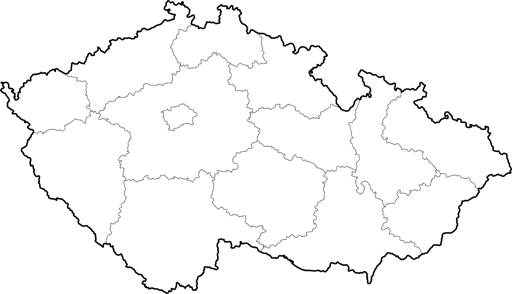
\includegraphics[width=0.5\textwidth]{files/map-coloring-czechia.png} \vfill
        
        \item Těžší instance  
        
        \vfill 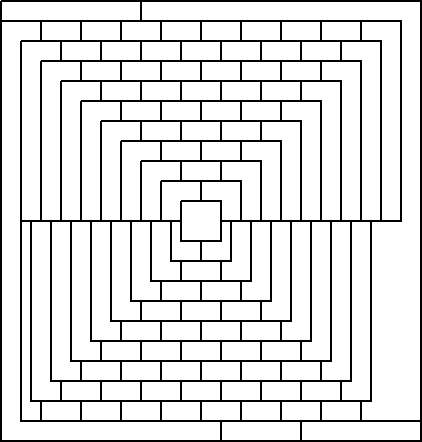
\includegraphics[width=0.33\textwidth]{files/map-coloring-hard.png} \vfill
    \end{enumerate}
    \end{multicols}

\end{problem}



\section*{K zamyšlení}
    
    
\begin{problem} 
    
    Pro danou formuli $\varphi$ v CNF najděte a 3-CNF formuli $\varphi'$ takovou, že $\varphi'$ je splnitelná, právě když $\varphi$ je splnitelná. Popište efektivní algoritmus konstrukce $\varphi'$ je-li dána $\varphi$ (tj. \emph{redukci} z problému SAT do problému 3-SAT).

\end{problem}


\begin{problem}
    Zakódujte problém setřídění dané $n$-tice celých čísel do SAT.
\end{problem}

\begin{problem}
    Zakódujte do SAT známou hádanku o farmáři, který potřebuje přepravit přes řeku vlka, kozu, a hlávku zelí.
\end{problem}

    
\end{document}